\documentclass[a4paper,12pt]{article}\usepackage[]{graphicx}\usepackage[]{color}
% maxwidth is the original width if it is less than linewidth
% otherwise use linewidth (to make sure the graphics do not exceed the margin)
\makeatletter
\def\maxwidth{ %
  \ifdim\Gin@nat@width>\linewidth
    \linewidth
  \else
    \Gin@nat@width
  \fi
}
\makeatother

\definecolor{fgcolor}{rgb}{0.345, 0.345, 0.345}
\newcommand{\hlnum}[1]{\textcolor[rgb]{0.686,0.059,0.569}{#1}}%
\newcommand{\hlstr}[1]{\textcolor[rgb]{0.192,0.494,0.8}{#1}}%
\newcommand{\hlcom}[1]{\textcolor[rgb]{0.678,0.584,0.686}{\textit{#1}}}%
\newcommand{\hlopt}[1]{\textcolor[rgb]{0,0,0}{#1}}%
\newcommand{\hlstd}[1]{\textcolor[rgb]{0.345,0.345,0.345}{#1}}%
\newcommand{\hlkwa}[1]{\textcolor[rgb]{0.161,0.373,0.58}{\textbf{#1}}}%
\newcommand{\hlkwb}[1]{\textcolor[rgb]{0.69,0.353,0.396}{#1}}%
\newcommand{\hlkwc}[1]{\textcolor[rgb]{0.333,0.667,0.333}{#1}}%
\newcommand{\hlkwd}[1]{\textcolor[rgb]{0.737,0.353,0.396}{\textbf{#1}}}%
\let\hlipl\hlkwb

\usepackage{framed}
\makeatletter
\newenvironment{kframe}{%
 \def\at@end@of@kframe{}%
 \ifinner\ifhmode%
  \def\at@end@of@kframe{\end{minipage}}%
  \begin{minipage}{\columnwidth}%
 \fi\fi%
 \def\FrameCommand##1{\hskip\@totalleftmargin \hskip-\fboxsep
 \colorbox{shadecolor}{##1}\hskip-\fboxsep
     % There is no \\@totalrightmargin, so:
     \hskip-\linewidth \hskip-\@totalleftmargin \hskip\columnwidth}%
 \MakeFramed {\advance\hsize-\width
   \@totalleftmargin\z@ \linewidth\hsize
   \@setminipage}}%
 {\par\unskip\endMakeFramed%
 \at@end@of@kframe}
\makeatother

\definecolor{shadecolor}{rgb}{.97, .97, .97}
\definecolor{messagecolor}{rgb}{0, 0, 0}
\definecolor{warningcolor}{rgb}{1, 0, 1}
\definecolor{errorcolor}{rgb}{1, 0, 0}
\newenvironment{knitrout}{}{} % an empty environment to be redefined in TeX

\usepackage{alltt}
\usepackage[applemac]{inputenc}
\usepackage[OT1,T1]{fontenc}

\setlength{\textwidth}{160mm}
\setlength{\textheight}{230mm}
\setlength{\oddsidemargin}{-5mm}
\setlength{\topmargin}{-10mm}
\usepackage{times}
\usepackage{setspace}
\usepackage{lscape}
\usepackage{amsmath,amssymb}
\usepackage{fancyvrb}
\usepackage{multirow}
\usepackage{float}
\usepackage{hyperref}
\usepackage{color}
\usepackage{listings}
\usepackage{fancyhdr}

\usepackage{fancyvrb,moreverb,boxedminipage}


\textwidth=6in
\textheight=8in
\topmargin=0.0in
\oddsidemargin=0in 
\baselineskip=18pt
\headheight=2cm
\setcounter{MaxMatrixCols}{10}

\newcommand{\ns}{\!\!\!}
\newcommand{\e}{\varepsilon}
\newcommand{\be}{\beta}
\newcommand{\s}{\sigma}
\newcommand{\vv}{\vspace{.5cm}}
\DeclareMathOperator{\plim}{plim}
\DefineVerbatimEnvironment{code}{Verbatim}{fontsize=\small}
\DefineVerbatimEnvironment{example}{Verbatim}{fontsize=\small}

\def\by{\mathbf{y}}
\def\bx{\mathbf{x}}
\def\ba{\mathbf{a}}
\def\bb{\mathbf{b}}
\def\be{\mathbf{e}}
\def\bu{\mathbf{u}}
\def\bv{\mathbf{v}}
\def\bz{\mathbf{z}}

%===========
%Greek letter vectors
%===========
\def\bbeta{\mbox{\boldmath $\beta$}}
\def\bgamma{\mbox{\boldmath $\gamma$}}
\def\bvareps{\mbox{\boldmath $\varepsilon$}}
\def\bleta{\mbox{\boldmath $\eta$}}
\def\bmu{\mbox{\boldmath $\mu$}}
\def\btheta{\mbox{\boldmath $\theta$}}
\def\bsigma{\mbox{\boldmath $\sigma$}}
\def\blambgam{\mbox{\boldmath $\lambda_{\gamma}$}}
\def\blambbet{\mbox{\boldmath $\lambda_{\beta}$}}
\def\blambda{\mbox{\boldmath $\lambda$}}

%===========
%Matrices
%===========
\def\bX{\mathbf{X}}
\def\bD{\mathbf{D}(\bsigma)}
\def\bV{\mathbf{V}(\bsigma)}
\def\bVinv{\mathbf{V}^{-1}(\bsigma)}
\def\bR{\mathbf{R}(\bsigma)}
\def\bA{\mathbf{A}}
\def\bB{\mathbf{B}}
\def\bZ{\mathbf{Z}}
\def\bIn{\mathbf{I_{N}}}
\def\bIm{\mathbf{I_{m}}}
\def\bIni{\mathbf{I_{n}}}
\def\SSW{\mathrm{SSW}}
\def\SSB{\mathrm{SSB}}
\def\Normal{\mathcal{N}\!}

%===========
%Parentheses, etc.
%===========
\def\op{\left(}
\def\cp{\right)}
\def\oc{\left[}
\def\cc{\right]}
\def\ok{\left\{}
\def\ck{\right\}}

%===========
%Statistical functions and real numbers.
%===========
\def\exE{\mathbb{E}}
\def\Real{\mathbb{R}}
\def\Var{\mathbb{V}ar}
\def\Proba{\mathbb{P}}

\hypersetup{colorlinks=true,linkcolor=blue,citecolor=blue, urlcolor=blue}
\urlstyle{tt}

\newenvironment{exercices}{\newcounter{moncompteur}\begin{list}
   {\bfseries Ex. \arabic{moncompteur}}{\usecounter{moncompteur}
     \setlength{\labelwidth}{2.6em}\setlength{\leftmargin}{3.1em}}}{\end{list}}
\renewcommand{\labelenumi}{\bfseries\alph{enumi})}
\newcommand{\splus}[3][0]{\texttt{>~#2}\ \ \ \ \textit{#3}\\[#1mm]}

\newenvironment{exo}
{\begin{center}\setlength{\textwidth}{140mm} \underline{Exercise:} \begin{minipage}[t]{120mm}}
{\end{minipage}\setlength{\textwidth}{160mm}\end{center}}


\usepackage{verbatim}

\lstset{ %
  language=R, 
  basicstyle=\ttfamily,
  backgroundcolor=\color{lightgray},   % choose the background color; you must add \usepackage{color} or \usepackage{xcolor}
  xleftmargin= 10 pt,
  xrightmargin= 10 pt,
  escapeinside={\%*}{*)},          % if you want to add LaTeX within your code
  frame=none,                    % adds a frame around the code
  numbers=none,                    % where to put the line-numbers; possible values are (none, left, right)
  numbersep=5pt,                   % how far the line-numbers are from the code
  numberstyle=\tiny\color{mygray}, % the style that is used for the line-numbers
  showspaces=false,                % show spaces everywhere adding particular underscores; it overrides 'showstringspaces'
}

\pagestyle{fancy}

\definecolor{mygreen}{rgb}{0,0.6,0}
\definecolor{mygray}{rgb}{0.5,0.5,0.5}
\definecolor{mymauve}{rgb}{0.58,0,0.82}
\definecolor{lightgray}{gray}{0.95}


%%%%%%%%%%%%%%%%%%%%%%%%%%%%%%%%%%%%%%%%%%%%%%%%%%%%%%%%%%%%%%%%%%%%%%%%%%%%
%
\IfFileExists{upquote.sty}{\usepackage{upquote}}{}
\begin{document}
%

\lhead{University of Geneva\\ \textbf{GLAM}\\
Prof. Eva Cantoni}
\rhead{GSEM\\ Spring 2022 \\ \textbf{Homework 03}}

\begin{center}
\bigskip

\bigskip

\bigskip

\bigskip

\bigskip

\bigskip

\fbox{{\Large Creating functions in \texttt{R} - Handout}}

\bigskip

\bigskip

\bigskip
\end{center}

%%%%%%%%%%%%%%%%%%%%%%%%%%%%%%%%%%%%%%%%%%%%%%%%%%%%%%%%%%%%%%%%%%%%%%%%%%%%


\setlength{\parskip}{1ex plus 0.5ex minus 0.2ex}
\parindent=0cm
\setlength{\parskip}{1ex plus 0.5ex minus 0.2ex}
\linespread{1.1}
\sloppy

\section{\underline{Exercise 1}}

% In this Exercise we would like you to write your own functions in \texttt{R}. The general procedure for defining new functions is as follows
% \begin{center}
% \begin{verbatim}
% myfun <- function(argument1,argument2,...){
%     expression1
%     expression2
% }
% \end{verbatim}
% \end{center}
% where \texttt{myfun} is the name of the function you are creating, \texttt{argument1,argument2,...} can be any type of \texttt{R} objects you are using as input and \texttt{expression} can be any computation and/or already existing function applied to the arguments. By default the result of the last expression is the returned value of the function. Consult the Help manual to learn more about writing your own functions.
% 
% \medskip

Write a function (name it \verb"mysummary") to compute and display the average and variance of a (vector) sample $\bx$, using functions such as
\verb"mean()", \verb"var()", \verb"return()" and \verb"list()"\footnote{Hint: you can look at \texttt{R} built-in functions as examples, by typing the name of the function in the console. Compare \texttt{median} and \texttt{mean}.}.

{\color{blue}
What follows is a proposition of a function that computes the wanted quantities. This function will return a \texttt{list} containing the results of the computations using the basic functions.  

\begin{knitrout}
\definecolor{shadecolor}{rgb}{0.969, 0.969, 0.969}\color{fgcolor}\begin{kframe}
\begin{alltt}
\hlstd{mysummary} \hlkwb{<-} \hlkwa{function}\hlstd{(}\hlkwc{x}\hlstd{)\{}
  \hlstd{res} \hlkwb{<-} \hlkwd{list}\hlstd{(}\hlkwd{mean}\hlstd{(x),}\hlkwd{var}\hlstd{(x),}\hlkwd{range}\hlstd{(x))}
  \hlkwd{names}\hlstd{(res)} \hlkwb{<-} \hlkwd{c}\hlstd{(}\hlstr{'mean of x'}\hlstd{,}\hlstr{'variance of x'}\hlstd{,}\hlstr{'min and max of x'}\hlstd{)}
  \hlkwd{return}\hlstd{(res)}
\hlstd{\}}
\end{alltt}
\end{kframe}
\end{knitrout}
In order to test our function, we shall create a vector of 100 observations drawn from a Standard Normal distribution on which, we will apply our function. We can store the results of this operation in an object named \texttt{my.sum} and retrieve its elements using the operator \$ and their respective names.
\begin{knitrout}
\definecolor{shadecolor}{rgb}{0.969, 0.969, 0.969}\color{fgcolor}\begin{kframe}
\begin{alltt}
\hlstd{x} \hlkwb{<-} \hlkwd{rnorm}\hlstd{(}\hlnum{100}\hlstd{)}

\hlstd{my.sum} \hlkwb{=} \hlkwd{mysummary}\hlstd{(x)}

\hlstd{my.sum[[}\hlnum{1}\hlstd{]]}
\end{alltt}
\begin{verbatim}
## [1] 0.1642238
\end{verbatim}
\begin{alltt}
\hlstd{my.sum}\hlopt{$}\hlstr{'mean of x'}
\end{alltt}
\begin{verbatim}
## [1] 0.1642238
\end{verbatim}
\begin{alltt}
\hlkwd{mysummary}\hlstd{(x)}\hlopt{$}\hlstr{'mean of x'} \hlcom{# since the result of our function is a list.}
\end{alltt}
\begin{verbatim}
## [1] 0.1642238
\end{verbatim}
\begin{alltt}
\hlkwd{mysummary}\hlstd{(x)[[}\hlnum{2}\hlstd{]]} \hlcom{# alternative way of retrieving the second element. }
\end{alltt}
\begin{verbatim}
## [1] 0.8144796
\end{verbatim}
\end{kframe}
\end{knitrout}
}

\section{\underline{Exercise 2}}


The goal of this exercise is to find numerical solutions of a set of estimating (score) equations and to compare them with those obtained with the \texttt{R} built-in functions.

Let's consider the \verb"breast-cancer-wisconsin.txt" dataset. We will use the response \verb"status" (coded 0/1) and only one explanatory variable  \verb"nuclei" (plus an intercept). 

We consider the logit function as the link between the random part $\exE[Y_i | \bx_i]$ and the systematic part (linear predictor) $\eta_i=\beta_0 + \beta_1 x_{i1}$.

Based on this, the formula for Newton-Raphson algorithm is:

\begin{align*}
\beta^{(k)}=
\beta^{(k-1)} +& 
\ok 
\sum_{i=1}^n 
\frac{\exp \op - \bx_i^T \beta^{(k-1)} \cp}{\oc 1 + \exp\op -\bx_i\beta^{(k-1)}\cp \cc ^2} 
\bx_i\bx_i^T
\ck ^ {-1}\\
&\times
\ok
\sum_{i=1}^n 
\oc 
y_i - \frac{1}{1 + \exp \op -\bx_i^T\beta^{(k-1)} \cp} 
\cc 
\bx_i 
\ck.
\end{align*}

\begin{enumerate}
%  \item Write the estimating (score) equations for the proposed model.
%  \item{Write the formulae for the Newton-Raphson algorithm and show that the ($2 \times 2$) matrix ${\mathcal J(\bbeta; \by)}$ is equal to $\sumin \exp(\bx_i^T\bbeta)(1+\exp(\bx_i^T\bbeta))^{-2} \bx_i \bx_i^T$.}
  \item{Write an \texttt{R} function that computes an update of the estimated parameters, given the previous value, according to the Newton-Raphson algorithm.}
  
{\color{blue}
  We build a function that computes \texttt{Ubeta}, which is $U(\beta, y)$ and \texttt{Jbeta} which is the Fisher information matrix.
    
\begin{knitrout}
\definecolor{shadecolor}{rgb}{0.969, 0.969, 0.969}\color{fgcolor}\begin{kframe}
\begin{alltt}
\hlstd{updatebeta} \hlkwb{<-} \hlkwa{function}\hlstd{(}\hlkwc{beta}\hlstd{,} \hlkwc{y}\hlstd{,} \hlkwc{X}\hlstd{)\{}
  \hlstd{eta} \hlkwb{<-} \hlkwd{as.vector}\hlstd{(X} \hlopt{%*%} \hlstd{beta)}
  \hlstd{Ubeta} \hlkwb{<-} \hlkwd{t}\hlstd{(X)} \hlopt{%*%} \hlstd{(y} \hlopt{-} \hlkwd{exp}\hlstd{(eta)} \hlopt{/} \hlstd{(}\hlnum{1} \hlopt{+} \hlkwd{exp}\hlstd{(eta)))}
  \hlstd{Jbeta} \hlkwb{<-} \hlkwd{t}\hlstd{(X)} \hlopt{%*%} \hlkwd{diag}\hlstd{(}\hlkwd{exp}\hlstd{(eta)} \hlopt{/} \hlstd{(}\hlnum{1} \hlopt{+} \hlkwd{exp}\hlstd{(eta))} \hlopt{^} \hlnum{2}\hlstd{)} \hlopt{%*%} \hlstd{X}
  \hlstd{beta} \hlopt{+} \hlkwd{solve}\hlstd{(Jbeta, Ubeta)}
\hlstd{\}}
\end{alltt}
\end{kframe}
\end{knitrout}
}

  \item\label{manually}{Taking the null vector as the starting value for $\bbeta$, perform a few iterations of the Newton-Raphson procedure using a \texttt{while()} in the following way:
  
  \begin{verbatim}
  while (max(abs(beta0-beta1))>tol & it<maxit){
  ...
  }
\end{verbatim}
  


where \texttt{beta0} and \texttt{beta1} are the actual and next beta estimations, \texttt{tol} is equal to $10^{-8}$ and \texttt{maxit} is $50$. Report the estimated $\bbeta$ in a table.}
  
{\color{blue} We first have to think about changing the \texttt{status} variable from (4/2) to (1/0). 

\begin{knitrout}
\definecolor{shadecolor}{rgb}{0.969, 0.969, 0.969}\color{fgcolor}\begin{kframe}
\begin{alltt}
\hlstd{breast} \hlkwb{<-} \hlkwd{read.table}\hlstd{(}\hlstr{"breast-cancer-wiconsin.txt"}\hlstd{,} \hlkwc{header}\hlstd{=}\hlnum{TRUE}\hlstd{)}

\hlstd{breast}\hlopt{$}\hlstd{status[}\hlkwd{which}\hlstd{(breast}\hlopt{$}\hlstd{status} \hlopt{==} \hlnum{4}\hlstd{)]} \hlkwb{<-} \hlnum{1}
\hlstd{breast}\hlopt{$}\hlstd{status[}\hlkwd{which}\hlstd{(breast}\hlopt{$}\hlstd{status} \hlopt{==} \hlnum{2}\hlstd{)]} \hlkwb{<-} \hlnum{0}
\end{alltt}
\end{kframe}
\end{knitrout}

Then we initialize our variables:

\begin{knitrout}
\definecolor{shadecolor}{rgb}{0.969, 0.969, 0.969}\color{fgcolor}\begin{kframe}
\begin{alltt}
\hlstd{y} \hlkwb{<-} \hlkwd{na.omit}\hlstd{(breast)}\hlopt{$}\hlstd{status} \hlcom{# responses in the model}
\hlstd{x} \hlkwb{<-} \hlkwd{cbind}\hlstd{(}\hlkwd{rep}\hlstd{(}\hlnum{1}\hlstd{,} \hlkwd{length}\hlstd{(y)),} \hlkwd{na.omit}\hlstd{(breast)}\hlopt{$}\hlstd{nuclei)}
\hlcom{#Construct the design matrix for our model}

\hlstd{tol} \hlkwb{<-} \hlnum{1e-8} \hlcom{# we set tol to an arbitrary value}
\hlstd{maxit} \hlkwb{<-} \hlnum{50} \hlcom{# same for maxit}
\hlstd{beta0} \hlkwb{<-} \hlkwd{c}\hlstd{(}\hlnum{0}\hlstd{,} \hlnum{0}\hlstd{)} \hlcom{#initialize the beta, could be set to any values}
\end{alltt}
\end{kframe}
\end{knitrout}

See \texttt{R} code lines 67-74 for the \texttt{while()} loop.

}

  \item{Write an \texttt{R} function that computes the log-likelihood of your model.}
  
  {\color{blue} Using the loglikehood expression of the Bernoulli distribution, be attentive to the fact that we introduce a minus sign because \texttt{optim()} minimizes by default}
  
\begin{knitrout}
\definecolor{shadecolor}{rgb}{0.969, 0.969, 0.969}\color{fgcolor}\begin{kframe}
\begin{alltt}
\hlstd{loglikelihood} \hlkwb{<-} \hlkwa{function}\hlstd{(}\hlkwc{beta}\hlstd{,} \hlkwc{x}\hlstd{,} \hlkwc{y}\hlstd{)\{}
  \hlstd{n} \hlkwb{<-} \hlkwd{nrow}\hlstd{(x)}
  \hlstd{loglike} \hlkwb{<-} \hlnum{0}
  \hlkwa{for} \hlstd{(i} \hlkwa{in} \hlnum{1}\hlopt{:}\hlstd{n)\{}
    \hlstd{etai} \hlkwb{<-} \hlopt{-}\hlstd{x[i, ]} \hlopt{%*%} \hlstd{beta}
    \hlstd{loglike} \hlkwb{<-} \hlstd{loglike} \hlopt{+} \hlstd{(}\hlnum{1} \hlopt{-} \hlstd{y[i])} \hlopt{*} \hlstd{etai} \hlopt{-} \hlkwd{log}\hlstd{(}\hlnum{1} \hlopt{+} \hlkwd{exp}\hlstd{(etai))}
  \hlstd{\}}
  \hlkwd{return}\hlstd{(}\hlopt{-}\hlstd{loglike)} \hlcom{# optim minimizes - we need to put a minus}
\hlstd{\}}
\end{alltt}
\end{kframe}
\end{knitrout}

  \item{Use the built-in function \verb"optim()" to solve the maximization problem (with the ``BFGS'' method). Compare your results with those in \textbf{b)}.}

{\color{blue} See lines 96-102 for details.  
}
\end{enumerate}

\section{\underline{Exercise 3}}

Consider the profile likelihood of page 112 of the course slides\footnote{Based on a handout by Professor David Patterson, University of Montana \url{http://www.math.umt.edu/patterson/}}: 
%
\begin{equation*}
    L_1\op\theta\cp = \underset{\mathbf{\delta}}{\mathrm{max}} \ L\op\theta, \mathbf{\delta} \cp, 
\end{equation*}
%
where $\theta$ is the parameter of interest of dimension 1, and $\delta$ is the
vector of the other model parameters. Under this formulation, we construct the following Likelihood
Ratio (LR) statistic to test $H_0 : \theta = \theta_0$: 
%
\begin{equation*}
    \mathrm{LR}\op \theta_0\cp = 
    2\oc \log L\op \widehat{\theta} , \widehat{\mathbf{\delta}}\cp - \log L\op \theta_0 , \widehat{\mathbf{\delta}}\cp\cc = 
    2 \oc \log L_1\op\widehat{\theta}\cp - \log L_1\op\theta_0\cp \cc \underset{H_0}{\sim}\chi^2_1,
\end{equation*}
%
where $\widehat{\theta}, \widehat{\mathbf{\delta}}$ are the maximum likelihood
(ML) estimators of $\theta$ and $\mathbf{\delta}$. The non-rejection region of
this test is determined by the condition $\mathrm{LR}\op\theta_0\cp < F^{-1}\op
1-\alpha\cp$, where $F$ is the cdf of the $\chi^2_1$ distribution, or
equivalently, all the $\theta_0$ such that: 
%
\begin{equation} \label{eq:nonrejection}
    \log L_1\op \theta_0\cp > \log L\op\widehat{\theta},\widehat{\mathbf{\delta}}\cp - \frac{1}{2}F^{-1}\op 1-\alpha\cp
\end{equation}
%
The points within the \emph{Profile Likelihood} CI will be those $\theta_0$ within the non-rejection region of the LR test.

Consider the goose permit data (file \texttt{goose.txt}) from Bishop and Heberlein (\textit{Amer. J. Agr. Econ.} 61, 1979), where 237 hunters were each offered one of 11 cash amount (bids) ranging from $1\$ $ to $ 200 \$ $ in return of their permits. We use a logit model with \texttt{log(bid)} as the explanatory variable (in addition to the intercept):
$$\log \op \frac{\pi_i}{1-\pi_i} \cp = \beta_0  + \beta_1 \log(\texttt{bid}_i) $$
where $\pi_i$ is the probability that a permit holder would accept bid amount $\texttt{bid}_i$.

%
\begin{enumerate}
    \item Estimate the parameters of the model, extract the log-likelihood with  \texttt{logLik()} to determine the cutoff value as in \eqref{eq:nonrejection} for $\alpha=0.05$ and $\alpha=0.01$. Compute the profiled likelihood CI for $\beta_1$ with the \texttt{confint()} function.

{\color{blue} As usual, we use the \texttt{glm()} function to obtain estimates of the model parameters.}



{\color{blue} When package \texttt{MASS} is loaded, the function \texttt{confint()} provides the desired PL confidence intervals, whereas the \texttt{confint.default()} yields the typical Normal (asymptotic) confidence intervals.}

\begin{knitrout}
\definecolor{shadecolor}{rgb}{0.969, 0.969, 0.969}\color{fgcolor}\begin{kframe}
\begin{alltt}
\hlstd{goose.plci.05} \hlkwb{=} \hlkwd{confint}\hlstd{(goose.glm,} \hlkwc{level}\hlstd{=}\hlnum{.95}\hlstd{)}
\end{alltt}


{\ttfamily\noindent\itshape\color{messagecolor}{\#\# Waiting for profiling to be done...}}\begin{alltt}
\hlstd{goose.nlci.05} \hlkwb{=} \hlkwd{confint.default}\hlstd{(}\hlkwc{object}\hlstd{=goose.glm)}
\hlkwd{cbind}\hlstd{(goose.plci.05, goose.nlci.05)}
\end{alltt}
\begin{verbatim}
##                 2.5 %    97.5 %      2.5 %    97.5 %
## (Intercept) -5.783372 -3.317595 -5.6807434 -3.224353
## log(bid)     0.978029  1.667461  0.9530795  1.639647
\end{verbatim}
\begin{alltt}
\hlstd{goose.plci.01} \hlkwb{=} \hlkwd{confint}\hlstd{(goose.glm,} \hlkwc{level}\hlstd{=}\hlnum{.99}\hlstd{)}
\end{alltt}


{\ttfamily\noindent\itshape\color{messagecolor}{\#\# Waiting for profiling to be done...}}\begin{alltt}
\hlstd{goose.nlci.01} \hlkwb{=} \hlkwd{confint.default}\hlstd{(}\hlkwc{object}\hlstd{=goose.glm,}\hlkwc{level}\hlstd{=}\hlnum{0.99}\hlstd{)}
\hlkwd{cbind}\hlstd{(goose.plci.01, goose.nlci.01)}
\end{alltt}
\begin{verbatim}
##                  0.5 %    99.5 %     0.5 %    99.5 %
## (Intercept) -6.2463329 -2.996867 -6.066670 -2.838426
## log(bid)     0.8875305  1.796307  0.845212  1.747514
\end{verbatim}
\end{kframe}
\end{knitrout}
    
    \item {\color{blue} In the following points, we intend to construct PL Confidence Intervals \emph{manually}.}

\begin{enumerate}
    \item Write an R code to compute the profile likelihood function $L_1(\beta_1)$ (which make use of the estimates of the previous point). 
    
    {\color{blue} Since the Profile Likelihood function is the maximization of the Likelihood with respect to one of the parameters while fixing the value of the other ones, we could think of using the \texttt{offset=...} argument in the \texttt{glm()} function. We could thus optimize the likelihood with respect to, say $\beta_0$, while fixing the value of $\beta_1$ by typing \texttt{offset = $\beta_1$} and redifining the \texttt{formula} so that it depends only on $\beta_0$. 
    
    Moreover, we could consider performing this optimization on a grid of values for $\beta_1$, and thus obtain values of the profile likelihood for this grid. The resulting values of the log-likelihood (extracted via \texttt{logLik()}) are thus the evaluations of the Profile Likelihood. (See the code).}



% {\color{blue} The values of the PL confidence intervals will be those in the grid whose evaluations are above the cutoff values, depending on the optimized likelihood and quantiles of the chi-squared distribution.}

\item Plot the profile likelihood $L_1(\beta_1)$ and the cutoff values.  

{\color{blue} In the following plot, we draw the PL function for both parameters. The values of the PL confidence intervals will be those in the grid whose evaluations are above the cutoff values, depending on the optimized likelihood and quantiles of the chi-squared distribution. For this illlustration, we have considered CI of levels 95\% and 99\%}

\begin{knitrout}
\definecolor{shadecolor}{rgb}{0.969, 0.969, 0.969}\color{fgcolor}
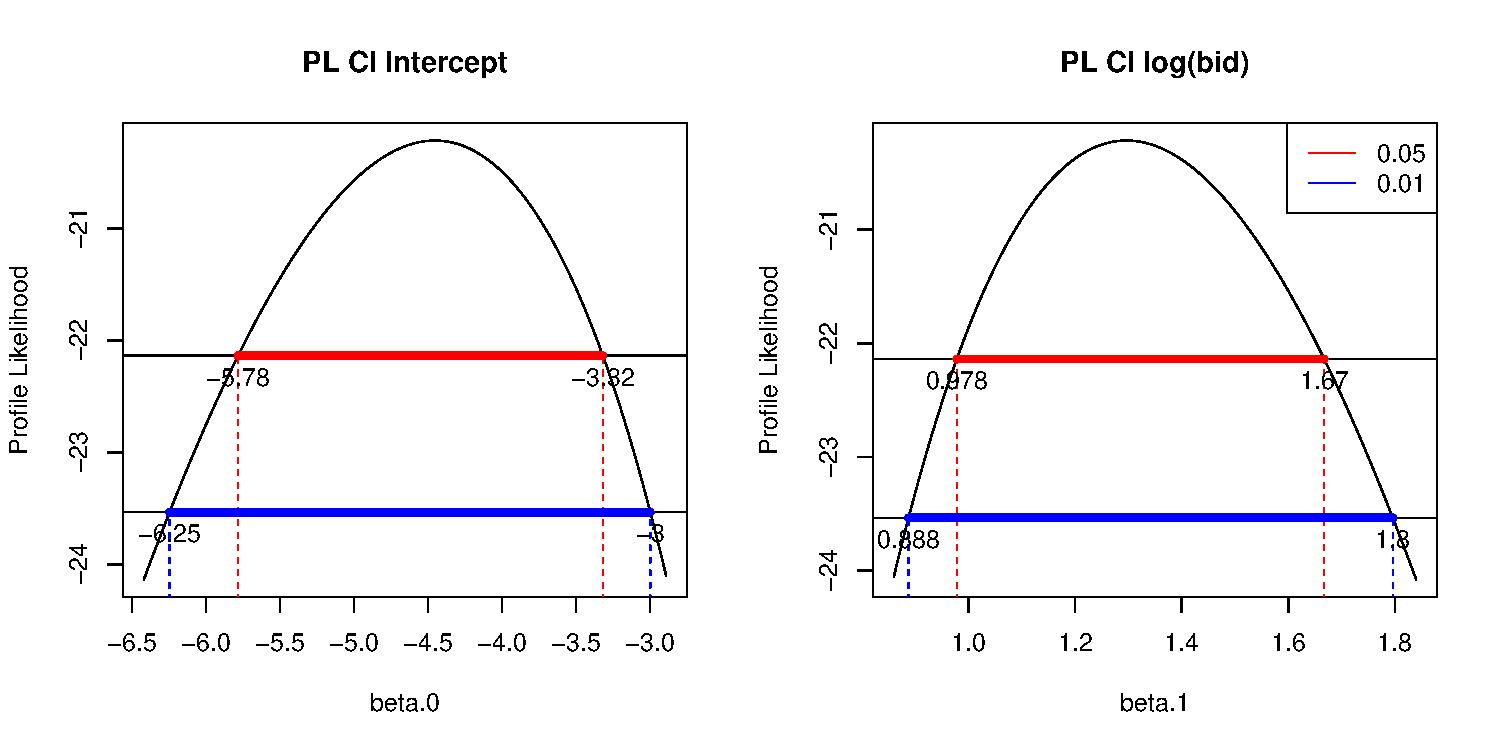
\includegraphics[width=\maxwidth]{figure/unnamed-chunk-10-1} 

\end{knitrout}

\item Compare the results with the CI computed at point \textbf{a)}.

{\color{blue} As we have said before, we can evaluate points in the grid and obtain the limits of the PLCI, by selecting the minimal (maximal) points in the grid such that their PL evaluations are beyond the cutoff rule. It is apparent that these values bare ressemblance to the ones obtained via the \texttt{confint()} method (improvements can be made by improving the grid).}

We compare obtained values for $\beta_0$
\begin{knitrout}
\definecolor{shadecolor}{rgb}{0.969, 0.969, 0.969}\color{fgcolor}\begin{kframe}
\begin{verbatim}
##                       2.5 %    97.5 %
## Intercept.plci.95 -5.783372 -3.317595
## Intercept.manl.95 -5.780000 -3.320000
##                       0.5 %    99.5 %
## Intercept.plci.99 -6.246333 -2.996867
## Intercept.manl.99 -6.240000 -3.000000
\end{verbatim}
\end{kframe}
\end{knitrout}

We compare obtained values for $\beta_1$
\begin{knitrout}
\definecolor{shadecolor}{rgb}{0.969, 0.969, 0.969}\color{fgcolor}\begin{kframe}
\begin{verbatim}
##                    2.5 %   97.5 %
## log_bid.plci.95 0.978029 1.667461
## log_bid.manl.95 0.980000 1.660000
##                     0.5 %   99.5 %
## log_bid.plci.99 0.8875305 1.796307
## log_bid.manl.99 0.8900000 1.790000
\end{verbatim}
\end{kframe}
\end{knitrout}

\end{enumerate}
\end{enumerate}

\end{document}
